% !Tex program = pdflatex

\documentclass[12pt,landscape]{article}
\usepackage{multicol}
\usepackage{calc}
\usepackage{ifthen}
\usepackage[landscape]{geometry}
\usepackage{amsmath,amsthm,amsfonts,amssymb}
\usepackage{color,graphicx,overpic}
\usepackage{hyperref}
\usepackage{enumitem}
\usepackage{upgreek}
\usepackage[italicdiff]{physics}
\usepackage{newtxtext,newtxmath}
\usepackage{mdframed}
\usepackage{amsbsy}

% This sets page margins to .5 inch if using letter paper, and to 1cm
% if using A4 paper. (This probably isn't strictly necessary.)
% If using another size paper, use default 1cm margins.
\ifthenelse{\lengthtest { \paperwidth = 11in}}
	{ \geometry{top=.5in,left=.5in,right=.5in,bottom=.5in} }
	{\ifthenelse{ \lengthtest{ \paperwidth = 297mm}}
		{\geometry{top=1cm,left=1cm,right=1cm,bottom=1cm} }
		{\geometry{top=1cm,left=1cm,right=1cm,bottom=1cm} }
	}

% Turn off header and footer
\pagestyle{empty}
 

% Redefine section commands to use less space
\makeatletter
\renewcommand{\section}{\@startsection{section}{1}{0mm}%
                                {-1ex plus -.5ex minus -.2ex}%
                                {0.5ex plus .2ex}%x
                                {\normalfont\normalsize\bfseries}}
\renewcommand{\subsection}{\@startsection{subsection}{2}{0mm}%
                                {-1explus -.5ex minus -.2ex}%
                                {0.5ex plus .2ex}%
                                {\normalfont\small\bfseries}}
\renewcommand{\subsubsection}{\@startsection{subsubsection}{3}{0mm}%
                                {-1ex plus -.5ex minus -.2ex}%
                                {1ex plus .2ex}%
                                {\normalfont\footnotessize\bfseries}}
\renewcommand\small{\@setfontsize\small{10}{11}}
\makeatother

% Define BibTeX command
\def\BibTeX{{\rm B\kern-.05em{\sc i\kern-.025em b}\kern-.08em
    T\kern-.1667em\lower.7ex\hbox{E}\kern-.125emX}}

% Don't print section numbers
\setcounter{secnumdepth}{0}


\setlength{\parindent}{0pt}
\setlength{\parskip}{1pt plus 0.5ex}

\newcommand{\tab}{\hspace*{1em}}
\newcommand{\ds}{\displaystyle}

% Redefine some commands for newtxmath boldness
\renewcommand{\grad}{\nabla}
\renewcommand{\curl}[1]{\nabla\times#1}
\renewcommand{\div}[1]{\nabla\cdot#1}
\renewcommand{\cross}{\times}
\newcommand{\defn}[1]{\textbf{Def} (\emph{#1})}
\newcommand{\thm}[1]{\textbf{Thm} (\emph{#1})}

\newcommand{\Var}[1]{\mathrm{Var}(#1)}
\newcommand{\Cov}[1]{\mathrm{Cov}(#1)}

\mdfsetup{skipabove=2pt,skipbelow=2pt, innertopmargin=-6pt, innerbottommargin=2pt, innerleftmargin=2pt, innerrightmargin=2pt}
\theoremstyle{definition}
\newmdtheoremenv{theorem}{Theorem}

% -----------------------------------------------------------------------

\begin{document}

\raggedright
\footnotesize
\begin{multicols}{3}

\raggedcolumns

% multicol parameters
% These lengths are set only within the two main columns
%\setlength{\columnseprule}{0.25pt}
\setlength{\premulticols}{1pt}
\setlength{\postmulticols}{1pt}
\setlength{\multicolsep}{1pt}
\setlength{\columnsep}{2pt}

\begin{center}
	\Large{\underline{ELEC 404 Formula Sheet}}
\end{center}

\section{Basic Concepts in RF Design}
Signal power in dBm:\\
\tab $\ds P_{\mathit{sig}\rvert\text{dBm}} = 10\log\left(\frac{P_\mathit{sig}}{1 \text{ mW}}\right)$

\subsection{Non-Linearity}
Peak 1-dB compression point:\\
\tab $\ds P_\text{1dB} = \sqrt{0.145\abs{\frac{\alpha_1}{\alpha_3}}}$

Input Third Intercept Point:\\
\tab $\ds A_\mathit{IIP3} = \sqrt{\frac{4}{3}\abs{\frac{\alpha_1}{\alpha_3}}}$\\
\tab $\ds \frac{A_\mathit{IIP3}}{P_\text{1dB}} \approx 9.6 \text{dB}$

Cascaded Non-Linear Stages:\\
\tab $\ds A_\mathit{IIP3} = \sqrt{\frac{4}{3}\left\vert\frac{\alpha_1\beta_1}{\alpha_3\beta_1 + 2 \alpha_1\alpha_2\beta_2 + \alpha_1^3 \beta_3}\right\vert}$\\
\tab $\ds \frac{1}{ A_\mathit{IIP3}^2} = \left\vert\frac{1}{ A_{\mathit{IIP3},1}^2} + \frac{3\alpha_2\beta_2}{2\beta_1} + \frac{\alpha_1^2}{A_{\mathit{IIP3},2}^2}\right\vert$\\
\tab $\ds \frac{1}{A_\mathit{IIP3}^2} \approx \frac{1}{A_{\mathit{IIP3},1}^2} + \frac{\alpha_1^2}{A_{\mathit{IIP3},2}^2} + \frac{\alpha_1^2\beta_1^2}{A_{\mathit{IIP3},3}^2} + \cdots$

\subsection{Noise}
Output Spectrum of a linear, time invariant system:\\
\tab $S_y(f) = S_x(f)\abs{H(f)}^2$

Resistor Noise Power Spectral Density:\\
\tab $\overline{V_n^2} = 4kTR \qquad \overline{I_n^2} = 4kTR$

MOSFET Noise Power Spectral Density ($\gamma \approx 2/3$):\\
\tab $\overline{V_n^2} = 4kT\gamma/g_m \qquad \overline{V_n^2} = 4kT\gamma g_m$

MOSFET $1/f$ noise corner frequency for some process constant $K$:\\
\tab $\ds f_c = \frac{K}{WLC_\mathit{ox}}\frac{g_m}{4kT\gamma}$

Noise Figure:\\
\tab $\ds \text{NF} = \frac{\mathit{SNR}_\mathit{in}}{\mathit{SNR}_\mathit{out}} \qquad \text{NF}|_\text{dB} = 10\log\left(\frac{\mathit{SNR}_\mathit{in}}{\mathit{SNR}_\mathit{out}}\right)$

Attenuation Factor:\\
\tab $\ds \alpha = \frac{Z_\mathit{in}}{Z_\mathit{in} + R_S}$

Noise figure as the total noise at the output divided by the noise at the output due to the source impedance ($\overline{V_n^2}$ is the output noise of device):\\
\tab $\ds \text{NF} = \frac{1}{\overline{V_\mathit{RS}^2}}\cdot\frac{\overline{V_\mathit{RS}^2}\abs{\alpha}^2A_v^2+\overline{V_n^2}}{\abs{\alpha}^2A_v^2} = 1 + \frac{\overline{V_n^2}}{\abs{\alpha}^2A_v^2}\cdot\frac{1}{\overline{V_\mathit{RS}^2}}$

Available power gain:\\
\tab $\ds A_P = \frac{\text{Power delivered to a matched load by stage}}{\text{Power delivered to a matched load by source}}$

Noise figure of cascaded stages (Friis' Equation):\\
\tab $\ds \text{NF}_\mathit{tot} = 1 + (\text{NF}_1 - 1) + \frac{\text{NF}_2 - 1}{A_{P1}} + \dots + \frac{\text{NF}_m - 1}{A_{P1}\cdots A_{P(m-1)}}$

\subsection{Passive Impedance Transformation}
Capacitor Quality Factor:\\
\tab $\ds Q_S = \frac{1}{R_SC\omega} \qquad Q_P = \frac{R_PC\omega}{1}$

Inductor Quality Factor:\\
\tab $\ds Q_S = \frac{L\omega}{R_S} \qquad Q_P = \frac{R_P}{L\omega}$

Series to Parallel Conversion $(Q_P = Q_S)$:\\
\tab $R_P = (Q_S^2 + 1)R_S$
\tab $\ds C_P = \left(\frac{Q_S^2}{Q_S^2 + 1}\right) C_S \qquad L_P = \left(\frac{Q_S^2 + 1}{Q_S^2}\right) L_S$

\subsection{Scattering Parameters}
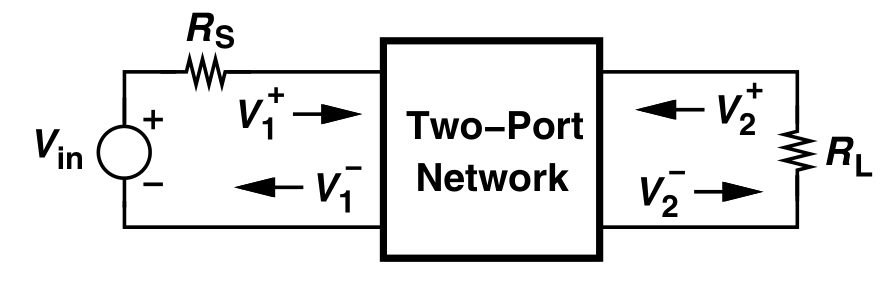
\includegraphics[width=\linewidth]{scattering_parameters.png}
\tab $V_1^- = S_{11}V_1^+ + S_{12}V_2^+$\\
\tab $V_2^- = S_{21}V_1^+ + S_{22}V_2^+$

Accuracy of input matching:\\
\tab $\ds S_{11} = \frac{V_1^-}{V_1^+}\rvert_{V_2^+ = 0} \approx \frac{Z_\mathit{in} - R_S}{Z_\mathit{in} + R_S}$

Reverse isolation:\\
\tab $\ds S_{12} = \frac{V_1^-}{V_2^+}\rvert_{V_1^+ = 0}$

Accuracy of output matching:\\
\tab $\ds S_{22} = \frac{V_2^-}{V_2^+}\rvert_{V_1^+ = 0} \approx \frac{Z_\mathit{out} - R_S}{Z_\mathit{out} + R_S}$

Circuit gain:\\
\tab $\ds S_{21} = \frac{V_2^-}{V_2^+}\rvert_{V_2^+ = 0}$

Scattering parameters in dB:\\
\tab $S_{mn\vert\text{dB}} = 20\log\abs{S_{mn}}$


% Footer content
\rule{0.3\linewidth}{0.25pt}
\scriptsize\\
Updated \today\\
\href{https://github.com/DonneyF/formula-sheets}{https://github.com/DonneyF/formula-sheets}
\end{multicols}%

\end{document}
